\begin{figure}[!htbp]
    \centering
    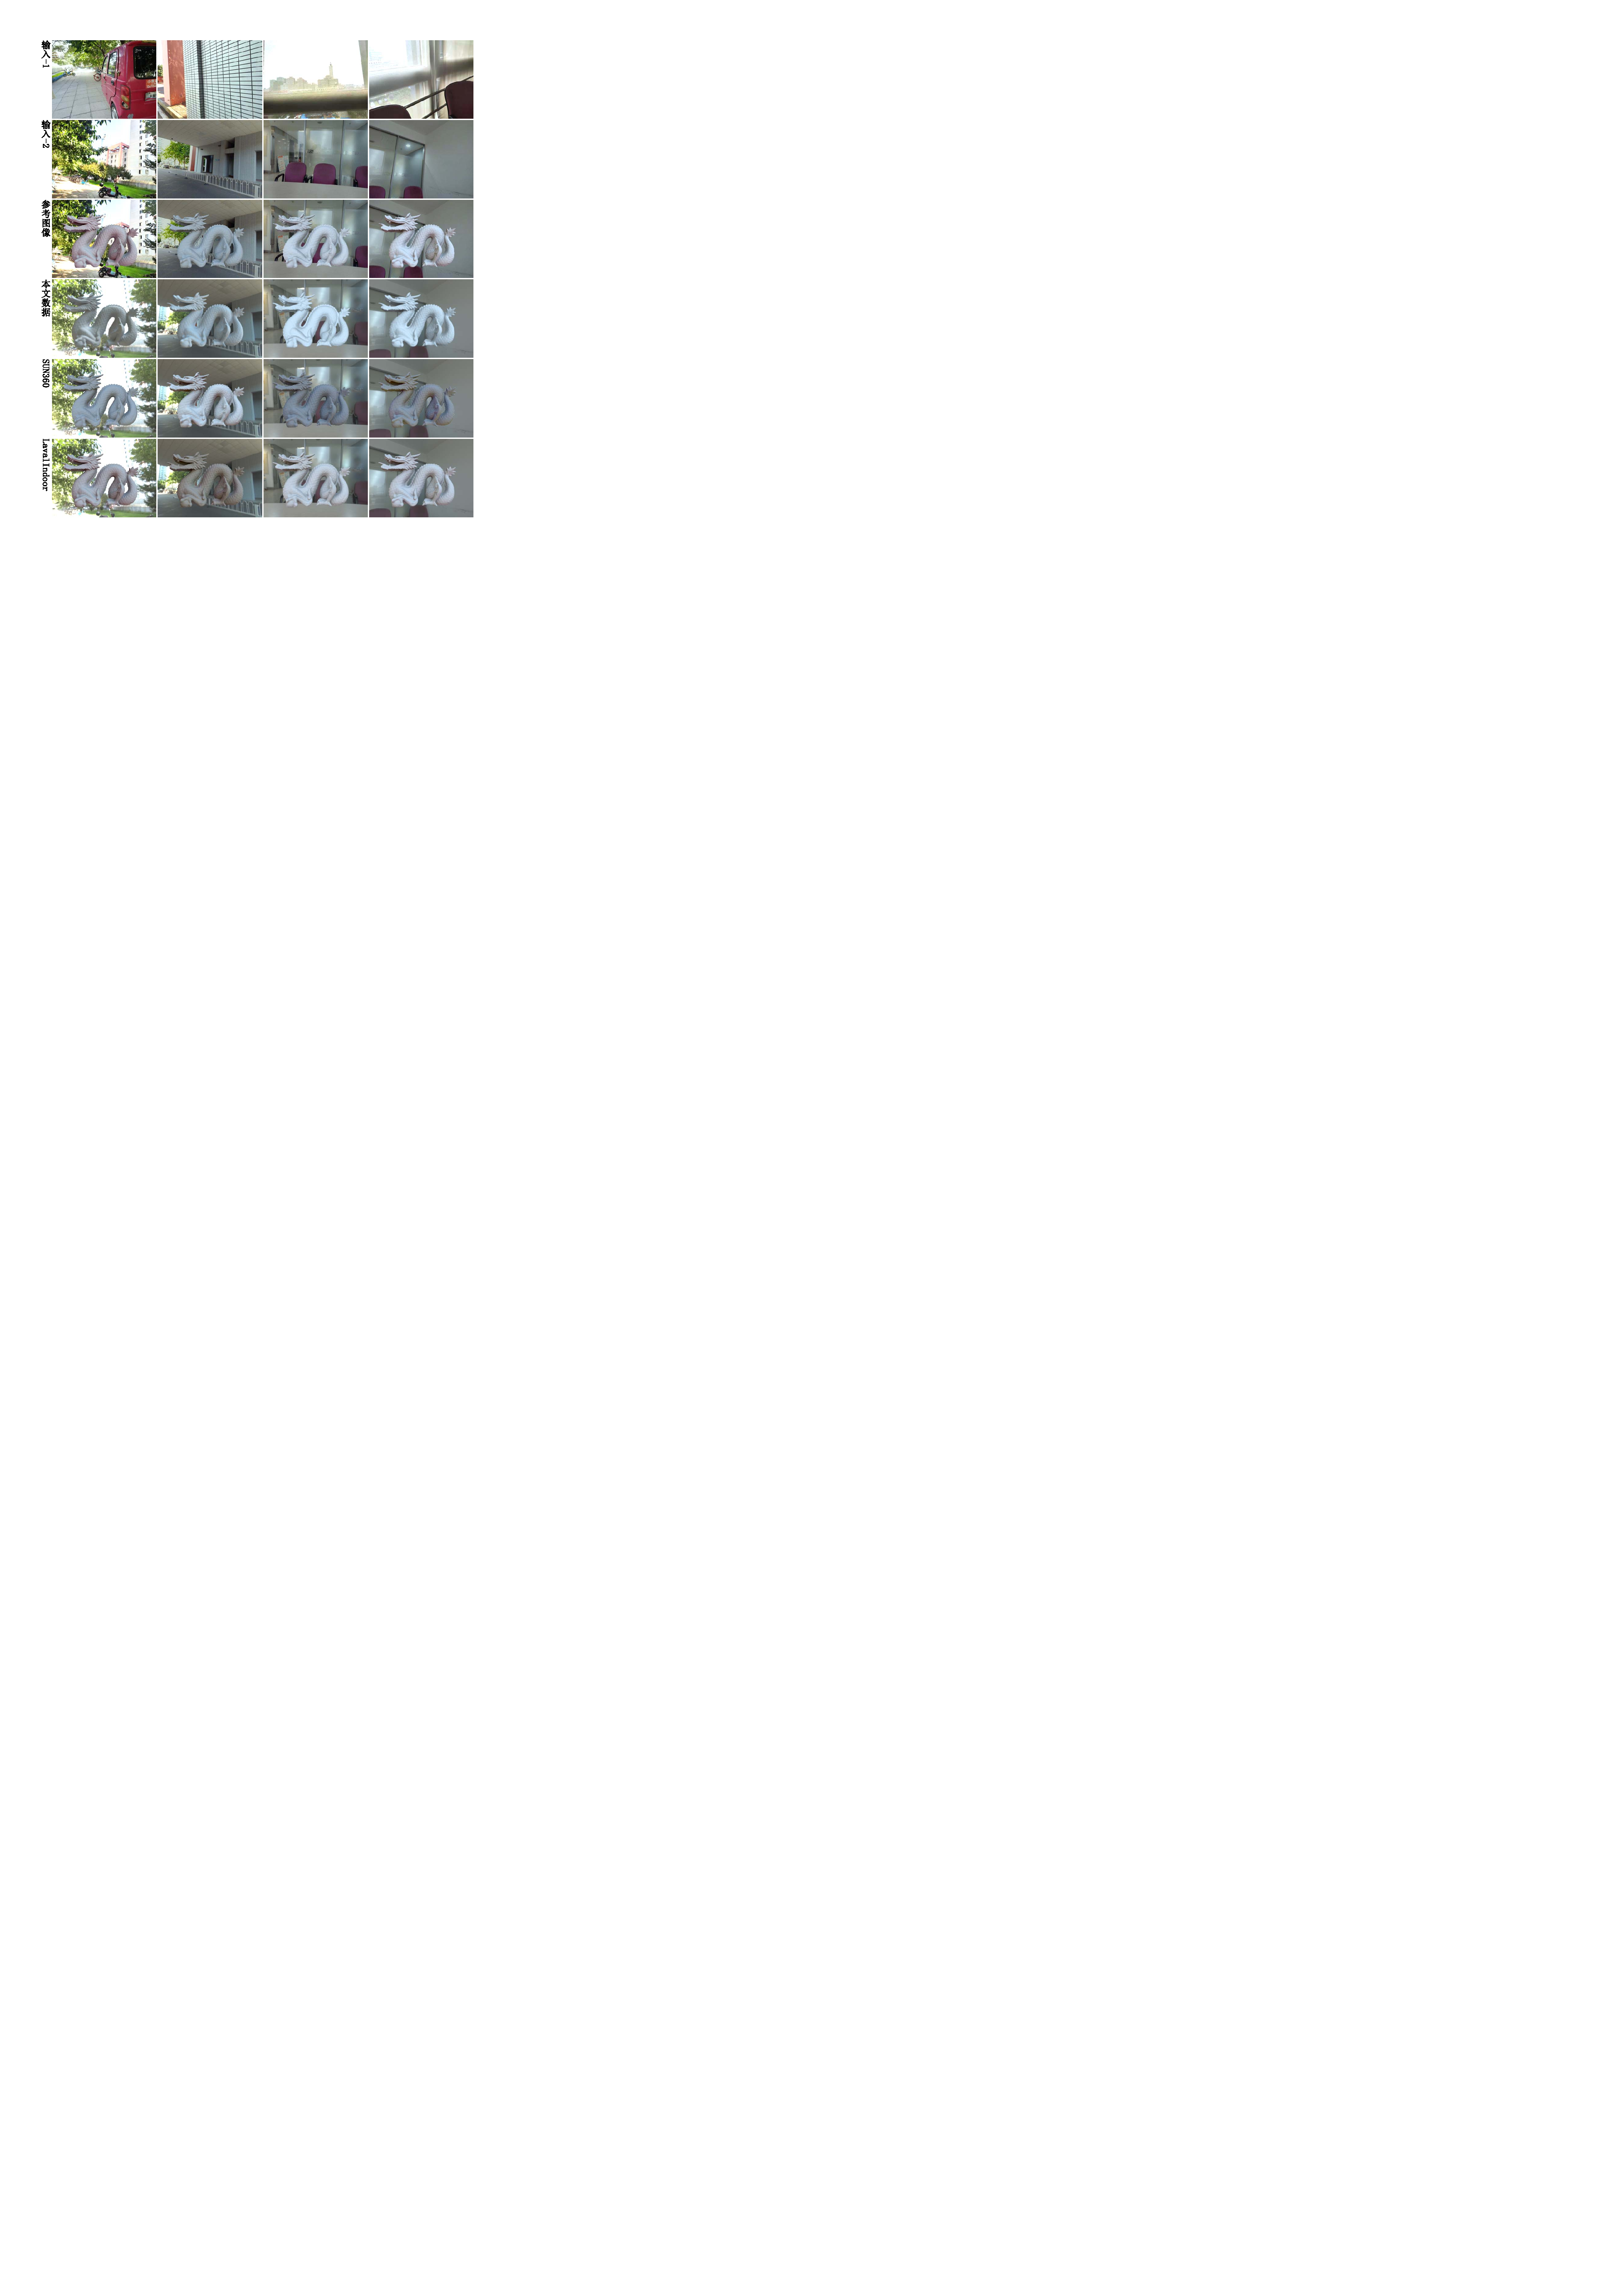
\includegraphics[width=0.98\textwidth]{Img/eval-data-previous.pdf}
    \caption[本文数据集与其它工作的可视化结果比较]
    {使用本文数据集训练的光照估计网络与其它工作在可视化结果的对比。可以看出使用本文数据集训练的网络,在室内外场景的结果明显优于其它两种数据集。另外从结果中可以看出,使用LAVAL数据集的结果在室内场景的表现中较为理想,在室外场景却得到了很差的结果,这是由于laval indoor数据集本身的局限性。此外,使用SUN360数据训练的光照估计网络,在较暗场景中的渲染结果与真实值较为接近(第二列),但明亮的场景中预测结果与真实值却相差甚远(第三、四列)。这也反映了低动态范围全景图本身的局限性,虽然在使用一定的光源探测技术将其拓展为HDR全景图,但这种HDR全景图却很粗糙,限制了其在光照估计问题中的作用。}
    \label{fig:eval-data-previous}
\end{figure}